\def\year{2020}\relax

\newcommand{\tuple}[1]{\ensuremath{\left \langle #1 \right \rangle }}


% These are the instructions for authors for IJCAI-19.

\newcommand{\qed}{\hfill\ensuremath{\blacksquare}}
\newcommand{\astar}{A$^*$}
\newcommand{\SAS}{SAS$^+$}
\newcommand{\wastar}{WA$^*$}
\newcommand{\arastar}{ARA$^*$}
\newcommand{\open}{\textsc{Open}}
\newcommand{\closed}{\textsc{Closed}}
\newcommand{\eff}{\textit{eff}}
\newcommand{\pre}{\textit{pre}}
\newcommand{\solvable}{\textit{S}}
\newcommand{\plannable}{\textit{P}}
\newcommand{\true}{\textit{T}}
\newcommand{\false}{\textit{$\bot$}}


%File: formatting-instruction.tex
\documentclass[letterpaper]{article} % DO NOT CHANGE THIS
\usepackage{aaai20}  % DO NOT CHANGE THIS
\usepackage{times}  % DO NOT CHANGE THIS
\usepackage{helvet} % DO NOT CHANGE THIS
\usepackage{courier}  % DO NOT CHANGE THIS
\usepackage[hyphens]{url}  % DO NOT CHANGE THIS
\usepackage{graphicx} % DO NOT CHANGE THIS
\urlstyle{rm} % DO NOT CHANGE THIS
\def\UrlFont{\rm}  % DO NOT CHANGE THIS
\usepackage{graphicx}  % DO NOT CHANGE THIS
\frenchspacing  % DO NOT CHANGE THIS
\setlength{\pdfpagewidth}{8.5in}  % DO NOT CHANGE THIS
\setlength{\pdfpageheight}{11in}  % DO NOT CHANGE THIS

\usepackage{subcaption} 
\usepackage[
backend=biber,
style=numeric,
citestyle=authoryear
]{biblatex}
\addbibresource{ref.bib} 

\usepackage{tabularx}
\usepackage{array}

\usepackage{booktabs}% for \toprule, \midrule, \bottomrule, and \cmidrule macros
\usepackage{amsmath} % for \text macro

%\usepackage[pdfencoding=auto]{hyperref}
\usepackage[draft]{hyperref}


\usepackage{amsmath}
\usepackage{booktabs}

\urlstyle{same}

\usepackage{algorithmic}

\usepackage[usenames,dvipsnames]{xcolor}
\usepackage[ruled,vlined,linesnumbered]{algorithm2e}
\usepackage{amsmath}
\usepackage{amsthm}
\usepackage{url}
\usepackage{multirow}
\usepackage[super]{nth}

\usepackage{xspace}


%
% Add comments in the text
%
\newboolean{showcomments}
%\setboolean{showcomments}{true}
\setboolean{showcomments}{false}

\ifthenelse{\boolean{showcomments}}
  {\newcommand{\nb}[3]{
  {\color{#2}\small\fbox{\bfseries\sffamily\scriptsize#1}}
  {\color{#2}\sffamily\small$\triangleright~$\textit{\small #3}$~\triangleleft$}
  }
  }
  {\newcommand{\nb}[3]{}
  }

\newcommand\Roni[1]{\nb{\textbf{Roni:}}{red}{#1}}
\newcommand\Omri[1]{\nb{\textbf{Omri:}}{orange}{#1}}


\newcommand{\inlinecite}[1]{\citeauthor{#1} \shortcite{#1}}

% \nocopyright
%PDF Info Is REQUIRED.
% For /Author, add all authors within the parentheses, separated by commas. No accents or commands.
% For /Title, add Title in Mixed Case. No accents or commands. Retain the parentheses.
 \pdfinfo{
/Title (Algorithm Selection for Optimal Classical MAPF)
/Author (Submission XXX)
} %Leave this	
% /Title ()
% Put your actual complete title (no codes, scripts, shortcuts, or LaTeX commands) within the parentheses in mixed case
% Leave the space between \Title and the beginning parenthesis alone
% /Author ()
% Put your actual complete list of authors (no codes, scripts, shortcuts, or LaTeX commands) within the parentheses in mixed case. 
% Each author should be only by a comma. If the name contains accents, remove them. If there are any LaTeX commands, 
% remove them. 

% DISALLOWED PACKAGES
% \usepackage{authblk} -- This package is specifically forbidden
% \usepackage{balance} -- This package is specifically forbidden
% \usepackage{caption} -- This package is specifically forbidden
% \usepackage{color (if used in text)
% \usepackage{CJK} -- This package is specifically forbidden
% \usepackage{float} -- This package is specifically forbidden
% \usepackage{flushend} -- This package is specifically forbidden
% \usepackage{fontenc} -- This package is specifically forbidden
% \usepackage{fullpage} -- This package is specifically forbidden
% \usepackage{geometry} -- This package is specifically forbidden
% \usepackage{grffile} -- This package is specifically forbidden
% \usepackage{hyperref} -- This package is specifically forbidden
% \usepackage{navigator} -- This package is specifically forbidden
% (or any other package that embeds links such as navigator or hyperref)
% \indentfirst} -- This package is specifically forbidden
% \layout} -- This package is specifically forbidden
% \multicol} -- This package is specifically forbidden
% \nameref} -- This package is specifically forbidden
% \natbib} -- This package is specifically forbidden -- use the following workaround:
% \usepackage{savetrees} -- This package is specifically forbidden
% \usepackage{setspace} -- This package is specifically forbidden
% \usepackage{stfloats} -- This package is specifically forbidden
% \usepackage{tabu} -- This package is specifically forbidden
% \usepackage{titlesec} -- This package is specifically forbidden
% \usepackage{tocbibind} -- This package is specifically forbidden
% \usepackage{ulem} -- This package is specifically forbidden
% \usepackage{wrapfig} -- This package is specifically forbidden
% DISALLOWED COMMANDS
% \nocopyright -- Your paper will not be published if you use this command
% \addtolength -- This command may not be used
% \balance -- This command may not be used
% \baselinestretch -- Your paper will not be published if you use this command
% \clearpage -- No page breaks of any kind may be used for the final version of your paper
% \columnsep -- This command may not be used
% \newpage -- No page breaks of any kind may be used for the final version of your paper
% \pagebreak -- No page breaks of any kind may be used for the final version of your paperr
% \pagestyle -- This command may not be used
% \tiny -- This is not an acceptable font size.
% \vspace{- -- No negative value may be used in proximity of a caption, figure, table, section, subsection, subsubsection, or reference
% \vskip{- -- No negative value may be used to alter spacing above or below a caption, figure, table, section, subsection, subsubsection, or reference


\usepackage{xspace}
\usepackage{acronym}

\usepackage{graphicx}
\graphicspath{ {images/} }

\setcounter{secnumdepth}{2} %May be changed to 1 or 2 if section numbers are desired.

% The file aaai20.sty is the style file for AAAI Press 
% proceedings, working notes, and technical reports.
%
\setlength\titlebox{2.5in} % If your paper contains an overfull \vbox too high warning at the beginning of the document, use this
% command to correct it. You may not alter the value below 2.5 in
%\title{Probabilistic Robust Multi-Agent Path Finding}
%Your title must be in mixed case, not sentence case. 
% That means all verbs (including short verbs like be, is, using,and go), 
% nouns, adverbs, adjectives should be capitalized, including both words in hyphenated terms, while
% articles, conjunctions, and prepositions are lower case unless they
% directly follow a colon or long dash

\newcommand{\OPEN} {{\textsc{Open}}}

\newtheorem{definition}{Definition}
\newtheorem{lemma}{Lemma}
\newtheorem{theorem}{Theorem}
\newcommand{\ignore}[1]{}

\author{Submission XXX}


%Written by AAAI Press Staff\textsuperscript{\rm 1}\thanks{Primarily Mike Hamilton of the Live Oak Press, LLC, with help from the AAAI Publications Committee}\\ \Large \textbf{AAAI Style Contributions by
%Pater Patel Schneider,} \\ \Large \textbf{Sunil Issar, J. Scott Penberthy, George Ferguson, Hans Guesgen}\\ % All authors must be in the same font size and format. Use \Large and \textbf to achieve this result when breaking a line
%\textsuperscript{\rm 1}Association for the Advancement of Artificial Intelligence\\ %If you have multiple authors and multiple affiliations
% use superscripts in text and roman font to identify them. For example, Sunil Issar,\textsuperscript{\rm 2} J. Scott Penberthy\textsuperscript{\rm 3} George Ferguson,\textsuperscript{\rm 4} Hans Guesgen\textsuperscript{\rm 5}. Note that the comma should be placed BEFORE the superscript for optimum readability
%2275 East Bayshore Road, Suite 160\\
%Palo Alto, California 94303\\
%publications20@aaai.org % email address must be in roman text type, not monospace or sans serif

\begin{document}




%%
%% The "title" command has an optional parameter,
%% allowing the author to define a "short title" to be used in page headers.
\title{Algorithm Selection for Optimal Multi-Agent Pathfinding}


%\author{}


%%
%% The "author" command and its associated commands are used to define
%% the authors and their affiliations.
%% Of note is the shared affiliation of the first two authors, and the
%% "authornote" and "authornotemark" commands
%% used to denote shared contribution to the research.

% \authornote{Both authors contributed equally to this research.}
% \email{trovato@corporation.com}
% \orcid{1234-5678-9012}
% \author{G.K.M. Tobin}
% \authornotemark[1]
% \email{webmaster@marysville-ohio.com}
% \affiliation{%
%   \institution{Institute for Clarity in Documentation}
%   \streetaddress{P.O. Box 1212}
%   \city{Dublin}
%   \state{Ohio}
%   \postcode{43017-6221}
% }

% \author{
% Eran Hershkovich,\textsuperscript{\rm 1}
% Roni Stern,\textsuperscript{\rm 1}
% Rui Abreu,\textsuperscript{\rm 1}
% Amir Elmishali,\textsuperscript{\rm 2}
% \textsuperscript{\rm 1}Ben Gurion University of the Negev,
% \textsuperscript{\rm 2}University of Lisbon\\
% eranhe@post.bgu.ac.il
% sternron@post.bgu.ac.il,
% rui@computer.org,
% amir9979@gmail.com,
% }

%\Eran{hope this is the right format}
\author{Submission \#}

\maketitle

%%
%% The abstract is a short summary of the work to be presented in the
%% article.
\begin{abstract}
At the past couple of years the research on multi-agent path finding (MAPF) has been flourishing, with new algorithms or algorithmic improvements appearing every year. 
In particular, although finding optimal solutions to MAPF is NP-Hard, there are to-date several successful algorithms that can find optimal solutions 
for problems with hundreds of agents. Nevertheless, it appears that no single MAPF algorithm dominates all benchmarks problems. 
Moreover, there are no clear, provable, guidelines for when each algorithm should be used. 
To address this, we apply a data-driven approach and propose the first successful algorithm selection method 
for optimal MAPF. Our algorithm selection method uses standard supervised learning algorithm with a set of hand-crafted MAPF-specific features and a customized weighting of the training instances. The results show that we are able to predict with very high accuracy the best algorithm to use for each instance. 
Using our algorithm selection method, we are able to achieve maximal coverage and running time over a range of maps and scenarios, compared to the state of the art. 
%The and machine learning techniques in order to automatically select the most suited solver for a given MAPF problem. We demonstrate the effectiveness of our method at being able to outperform any individual MAPF algorithm on MAPF benchmarks.
\end{abstract}

%%
%% This command processes the author and affiliation and title
%% information and builds the first part of the formatted document.

\section{Introduction}

% Algorithm selection has been used in other places
Algorithm selection methods became an effective tool for boosting problem solving performance. This approach has pushed the state-of-the-art in satisfiability (\cite{xu2008satzilla} and constrained programming (\cite{o2008using}), especially due to the fact that there is no single solver which dominate across a wide range of problem instances.

% From single agent to MAPF
Path finding is a classic problem in AI. Path finding problems for a single agent can usually be effectively solved using the \astar  algorithm (\cite{appi1966formal}). Unfortunately, multi agent path-finding problems become intractable when solved using the classical single agent path finding algorithms. The multi-agent path finding (MAPF) problem consists of a graph and a number of agents. Each agent has start and goal positions. At each time step an agent can either move to a neighboring location or can wait in its current location, while avoiding conflicts with other agents (i.e., without being in the same location at the same time or crossing the same edge simultaneously in opposite directions) 
MAPF has practical applications in robotics, video games, vehicle routing etc. (\cite{silver2005cooperative}; \cite{dresner2008multiagent}). In its general form, MAPF is NP-complete, because it is a generalization of the sliding tile puzzle which is known to be NP-complete (\cite{ratner1986finding}).

% Our contribution
The contribution of this paper is demonstrating the effectiveness of utilizing basic domain knowledge of classical MAPF algorithms in order to extract features from a MAPF problem. Then, using those features to build a GDBT model to perform algorithm selection which significantly outperform the use of any single algorithm. Furthermore, this paper explores current MAPF algorithms weakness and strengths according using explainabillity methods on the machine learning model trained for the task of algorithm selection 

\section{Background}








Recently, a comprehensive survey on algorithm selection methods (for combinatorial search problems) provided by \cite{hutteralgorithm} . 

TODO: Add background on development of different MAPF solvers
TODO: Add background on algorithm selection methods, as SATZilla 

\section{Problem Definition}
Although there was a development in algorithm selection, especially since (\cite{xu2008satzilla}), there were no attempts at utilizing algorithm selection techniques in order to select the most suitable algorithm for a classical MAPF (as defined by \cite{stern2019multiagent}) problem. At this section, we will define the task of algorithm selection in the context of classical MAPF problems.

\subsection{Classical MAPF}
We will use the term Classical MAPF problem, as described by \cite{stern2019multiagent}. Classical MAPF problem with k agents is defined by a tuple $\langle G,s,t \rangle$, where G = (V,E) is an un-directed graph, s: [1....,k] $\rightarrow$ V maps an agent to a source vertex, and t: [1,...,k] $\rightarrow$ V maps an agent to a target vertex.
At Classical MAPF, time is assumed to be discrete, and in every time step each agent is situated in one of the graph vertices and can perform a single action. An action defined by the function a: V $\rightarrow$ V, such that a(v) = $\hat{v}$ means that if an agent at vertex v and performs a then it will be in vertex $\hat{v}$ in the next time step. Each agent has twp types of actions: wait and move. A wait action means that the agent stays in it's current vertex another time step. A move action means that the agent moves from its current vertex v to an adjacent vertex $\hat{v}$ in the graph.
For a sequence of action $\pi$ =($a_1,...,a_n$) and an agent i, we denote by $\pi_i$[x] the location of the agent after executing the first x actions in Pi, starting from the agent's source s(i).


\subsection{Algorithm Selection}
We refer to algorithm selection as the classic problem of selecting the best algorithm from a given set of algorithms on a per-instance basis, as defined by \cite{rice1976algorithm}. Although research for new MAPF algorithms is evolving, we follow the No Free Lunch (NFL) theorem (\cite{wolpert1997no}) at this paper, which states that high-performing algorithms must in some way fit a specific problem space, but in other problem spaces will be outperformed by other algorithms. Therefore, we choose to apply algorithm selection in order to select the best algorithm for each MAPF problem, thus stepping towards gaining better understanding of MAPF problems. \Roni{I am not sure this is correct usage of NFL.}

Specifically, for classic MAPF domain, we demonstrate the dramatic importance of accurate algorithm selection, using Fig 1. 

\begin{figure}[h]
    \centering
    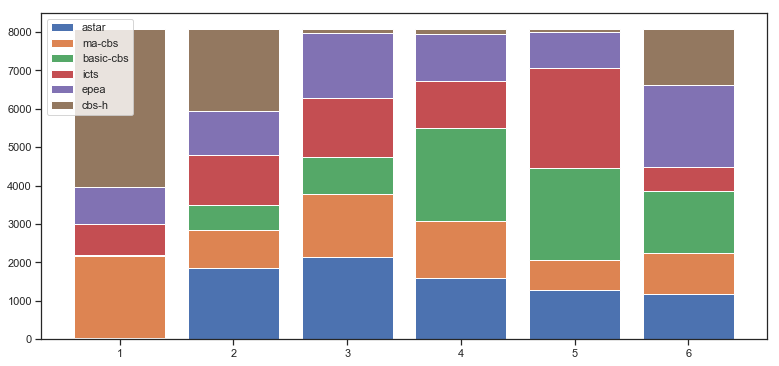
\includegraphics[width=0.5\textwidth]{images/stacked_bar_rankings.JPG}
    \caption{Each column at figure 1 visualize the relation between the solvers for a given rank. We can see that while MA-CBS is superior (solved fastest, thus ranked 1) more times than the others - it is obviously inferior at some cases, which might be costly in terms of solving a wide range of problems. Indeed, other more "stable ranked" algorithms will solve the entire problems at MovingAI dataset significantly faster. \Roni{Text is incorrect}}
    \label{fig:1}
\end{figure}







\section{Proposed Approach}

% Effort estimation vs. direct algorithm selection

% Features 

% Training set selection

% Algorithmic details


\section{Experimental Results}

% Overall results

% Cactus per map

% Feature importance

\section{Discussion and Conclusion}







\section{Proposed Approach}
Our approach leverages basic domain knowledge on classical MAPF problems, and recent advances in GDBT. We extract features for each MAPF problem, and train a regression model \Roni{No, this is just one of the approaches} to predict the running time for each algorithm on a given MAPF problem. We evaluate our work relatively to an oracle selection of algorithm, and to recent deep learning based methods for algorithm selection, as examined by \cite{sigurdson2017deep}, \cite{sigurdson2019deep} for pathfinding domain and  \cite{loreggia2016deep} for CSP domain.

At this section we will give overview on the MAPF feature extraction, our set of MAPF algorithms and set of MAPF problems. Then will give details on our way to select the learning model.

\subsection{MAPF Problems}
We decided to rely on the publicly available benchmark \footnotemark, due to its wide variety of MAPF problems. As described at (\cite{sturtevant2012benchmarks}), it contains 28 maps that represent the following grids:
\begin{itemize}
  \item \textbf{Games} - Using maps from video games is common at the field of MAPF solvers. Moving AI dataset contains 10 different game maps.
  \item \textbf{Cities} - 3 city maps (Berlin, Boston, Paris) 
  \item \textbf{Maze} - 4 maze maps.
  \item \textbf{Room} - 3 room maps.
  \item \textbf{Random} - 4 random maps.
  \item \textbf{Empty} - 4 empty (no obstacles) maps.
\end{itemize}

Due to the extreme runtime variation often exhibited by algorithms for solving MAPF problems, it is common practice to terminate unsuccessful runs after they exceed a so-called captime.
We choose 5 minutes as the captime.
When all solvers failed on a MAPF problem, we decided to discard it from the dataset used for training the model, after experimenting with both options (include/exclude the MAPF problems which all solvers failed on) and observed that the marginal error from the oracle solver was not effected. 

Each map at this benchmark has 25 different scenarios. A scenario is the specific placement of agent's start and goal positions. Each scenario is solved incrementally, in a way that we solve for one agent, two agents and continue until no solver able to solve under the configured captime (i.e., 5 minutes). 

\subsubsection{Splitting Data}
It is well known that in order to build a model with good generalization performance, a sensible data splitting strategy is crucial. Specifically, splitting MovingAI benchmark isn't a trivial task, due to the fact that the scenarios are solved incrementally. Thus, while splitting the dataset, we validated that data from a given scenario must not be splitted between train and test sets. Thus, we used 30\% of the scenarios as the held-out test set.

\footnotetext{https://movingai.com/benchmarks/mapf.html}

% TODO: do we really need to run 3 times? is there randomness in the solvers? Not that I know of... NEED TO DECIDE BEFORE RUNNING MOVINGAI

\subsubsection{Dealing with censored data}

As mentioned above, we censored the running time of each algorithm to 5 minutes. Methods to deal with censored data in the context of machine learning models studied in the context of survival analysis from actuarial science. Specifically, (\cite{schmee1979simple}) described an iterative method for handling censored data in regression models. We experimented with the next options: 1. Using \cite{schmee1979simple} method, 2. Treat censored data as uncensored, 3. Drop censored data.

Surprisingly, the second option achieved the best results at our experiments. 
Omri: TODO. Roni, do we need to write the results for each option? \Roni{Ideally yes, but not now.}

\subsection{Evaluated Algorithms}
We selected a set of high-performance MAPF solvers, while aiming for a diverse set such that the solvers running times would be significantly different throughout the data set, thus motivating the importance of learning to precisely select the best algorithm for each MAPF problem. Also, we picked our solvers such that they have relatively uncorrelated running times, due to their different strategies to solve MAPF problems.

The following set of evaluated algorithms used in this work are:

\subsubsection{ \astar with OD and ID}
(\cite{standley2010finding} \cite{standley2012independence})
 TODO TODO TODO TODO TODO TODO TODO TODO TODO 
\subsubsection{ Enhanced Partial Expansion \astar }  (\cite{goldenberg2014enhanced})
TODO TODO TODO TODO TODO TODO TODO TODO TODO TODO 
\subsubsection{ CBS } 
(\cite{sharon2015conflict}/)
TODO TODO TODO TODO TODO TODO TODO TODO TODO TODO TODO 
\subsubsection{ Meta Agent CBS }
(\cite{sharon2012meta})
TODO TODO TODO TODO TODO TODO TODO TODO TODO TODO TODO 
\subsubsection{ CBS-H }
TODO TODO TODO TODO TODO TODO TODO TODO TODO TODO TODO 
\subsubsection{ Increasing Cost Search Tree } (\cite{sharon2013increasing})
TODO TODO TODO TODO TODO TODO TODO TODO TODO TODO TODO 


\subsection{Feature Extraction}
In order to train a model, we needed to decide what are the features or
characteristics of the MAPF problem that are likely to correlate with algorithm performance? We experimented both with manually extraction of features and automatic extraction using deep learning models, inspired by \cite{sigurdson2019deep} and also using graph embedding (CITE graph2vec) approaches to generate features. At this section we will give details about the manually extracted features, and elaborate on other approaches while comparing results at Section 5.

\subsubsection{Manually Extracted Features} We define a small set of features represent the MAPF problem. Defining a small set of relatively simple-to-compute features enable our method to be effective. The features extracted for MAPF problem defined at Table 1.

We aimed at extracting features based on our domain knowledge of the examined algorithms. Therefore, we extracted features that will describe the grid (GridRows,GridColumns,NumOfObstacles,ObstacleDensity,Sparsity) and features that will describe the agents (BranchingFactor, NumOfAgents) and features that will reveal high-level information about the locations of the agents on the grid (AvgDistanceToGoal, MaxDistanceToGoal, MinDistnaceToGoal, AvgStartDistances, AvgGoalDistances, PointsAtSPRatio, Sparsity)

\begin{center}
\begin{table}[t]
\begin{tabular}
{|c | c|}
\hline
Name & Description \\ 
\hline\hline
GridRows & \#Rows at grid \\
\hline
GridColumns & \#Cols at grid \\
\hline
NumOfAgents & \#Agents at grid \\
\hline
NumOfObstacles & \#NumOfObstacles \\
\hline
BranchingFactor & $\#Actions^{\#Agents}$ \\
\hline
ObstacleDensity & $\frac{\#NumOfObstacles}{\#Rows\#Cols}$ \\
 \hline
AvgDistanceToGoal & Average distance of all agents to goal \\
 \hline
MaxDistanceToGoal & Maximum distance to goal \\
 \hline
MinDistanceToGoal & Minimum distance to goal \\
 \hline
AvgStartDistances & Average distance between all start positions \\
 \hline
AvgGoalDistances & Average distance between all goal positions \\
 \hline
PointsAtSPRatio & $\frac{\#Agents}{\#Row\#Cols - \#NumOfObstacles}$ \\
 \hline
Sparsity & TBD \\
 \hline
\hline
\end{tabular}
\label{table:1}
\caption{A list of extracted features for every MAPF problem. "PointsAtSPRatio" is the Ratio of points that are on a shortest path of an agent to the total number of points. }
\end{table}
\end{center}

\subsection{Learning objective}
Algorithm selection problem might be solved as classification (CITE), regression (CITE) and ordinal regression (CITE) problems (including variations of multi-output models). Choosing the right objective is crucial, and should take into considerations multiple issues:
1. Wrong selection costs are not the same for different
errors (it is clear that selecting the slowest algorithm should be more penalised than selecting the second-fastest algorithm).
\Roni{Well, we currently do not make use of this in an effective way, right? the weighting did not affect the results}
2. Some problems may be solved at the same order of magnitude of time across all solvers, and some problems might have large margin between running time of different solvers, therefore the learning objective should take into consideration the variance of the solvers running time.
3. Predicting running times directly (at milliseconds) considered a noisy target for regression models. 

Ordinal regression methods, recently reviewed in details by \cite{gutierrez2015ordinal}, might look like an elegant way to bypass the direct learning of running times, by training a model to predict the order of algorithms in respect to their running times on each problem. Yet, it is well-known that prior knowledge about the pair-wise class distances (i.e., the distance between fastest and second-fastest solvers) has significant effects on performance, as shown by \cite{sanchez2013exploitation}. Thus, at this paper we explore only classification and regression approaches.

Choosing between classification and regression can be thought of as choosing between metrics at the algorithm selection domain (i.e., prioritize accuracy or minimum running time). Therefore we aim to balance between running time and accuracy while training our model.

TODO: Add figure to show relation between accuracy and coverage. 


At the field of meta-learning, algorithm selection methods (CITE) attempts to identify the most suitable classifier (and parameter settings) for a given classification problem. Recent advances at this field explores the balancing between accuracy of the selected classifier and the training time it took to train it (\cite{brazdil2003ranking}, \cite{}, cite{}). Inspired by their methods, at this paper we detail our methods to balance between accuracy and running time at the field of MAPF algorithm selection.

\subsubsection{Multi Task Training}
Train one model with two tasks - predict the runtime for each algorithm + classify the best algorithm. Specify about loss weights.
Give in short details about training the CNN while trying to predict the extracted features.

\subsubsection{Relative Runtime As Probability}
TODO: explain on a method: Normalize the outputs to be probability distribution for each example and use classification with log softmax output and cross enropy loss.
For example - If for a given instance the results of algorithms was: 1. 10 mili, 2. 11 mili, 3. 100 mili, 4. 1000 mili, 5. 180000 mili, then the target for the classification problem will be the normalized probability (1 - relative part of time to sum of al time), and using the log softmax activation (log in order to not be biased towards the max) to predict this probability distribution. Thus effectively the balancing between accuracy (fastest solver thus highest probability) and coverage (never pick low probability because high loss) is achieved. 
Why this balancing not achieved using regression? Because regression have multiple problems (censored data, "noisiness" regarding to scale of miliseconds..)
\Roni{Do we have experiments for this?}


\subsubsection{Experiment with SATZilla2012 cost-sensitive learning approach}
\cite{xu2012satzilla2012} used cost-sensitive binary classification model for every pair of solvers. Then, at prediction, they used those classifiers as selecting the solver with the highest number of votes (i.e., highest number of times being predicted). We experimented with this approach and did not seen improvement. Thus, due to the large time it takes to train all pairs and the fact that it didn't gave us better results, we don't use this method.

\subsubsection{Sample Weight}
It is well understood that not all MAPF problems are equally important. Some MAPF problems might be solved very fast by all solvers, and some might be solved very slow. In both of those cases, the gain of using algorithm selection is relatively small, thus during training we want to give more weight to the MAPF problems where the divergence between running times of different solvers is high. Therefore, we set the weight of MAPF problem $i$, $W_i$, to be the standard deviation of running times :

$W_i =  \sqrt{\frac{1}{N-1} \sum_{j=1}^N (r_i,j - \overline{r_i})^2}$, 
% log{\sigma_i}$, $\sigma_i =

where N=5 number of solvers used at this paper, $\overline{r_i}$ denotes the average running time of all solver on problem i and $r_ij$ denotes running time of algorithm j on problem i.

% np.log10(np.std(x[only_alg_runtime_cols].values)

\subsubsection{Hardness models}
TODO: Explain about experiments with hardness binary models - a binary classifier if a problem is "hard" or not for each solver, and a regression for "hard" problems and "easy" problems for each classifier.

\subsubsection{Meta Model}
TODO: Explaing about experiments at using regression model outputs as inputs to the classifier model.

\subsubsection{Log Runtime}
A common practice when performing regression to predict runtime is using log transformation, due to the large variance in runtimes for hard pathfinding problems.  

\subsection{Learning models}
In order to learn to select between the MAPF algorithms, we experimented with three different learning approaches: Gradient Boosting, Convolution neural networks, and graph embedding techniques.

\Roni{Not clear what we actually did and what we just played around with}

\subsubsection{Gradient Boosting}
TODO
\subsubsection{Convolution Neural Networks}
\cite{sigurdson2019deep} used convolution neural networks (CNN) to address the algorithm selection problem for online MAPF. In order to compare our model with their approach, we followed their approach for generating the input images: blocked and unblocked nodes are represented by white and black pixels, respectively. Each agent start and goal location indicated with a greed and red pixel, respectively. 

Although we believe better image representation (i.e., representing shortest path for each agent) might give better results, at this paper we will train the CNN followed by their approach for comparison.

\subsubsection{Graph embedding}
TODO

\subsection{Evaluation Metrics}
In order to compare the results of our learning model, we define the following evaluation metrics

\subsubsection{Accuracy}
An accurate prediction for a given MAPF problem, is a prediction of the fastest algorithm. Accuracy is the percentage of samples (MAPF problems) that our model predicted an accurate prediction for them.

\subsubsection{Sum of costs}
In the context of Classical MAPF evaluation metrics, sum of costs is common when evaluating a solution to a given MAPF problem. 
We define sum of costs for an algorithm selection model as the sum of running times it took to solve a set of problems. 
Sum of costs for an algorithm selection model M, over set of problems $\Omega$, given a running time function T, which returns the running time of solving a problem using a solver, defined as:\medskip
$\sum_{p}^{\Omega} T(M(p), p)$
Where $M(p)$ is the model prediction of a solver, and $T(M(p),p)$ is the running time the predicted solver took to solve the problem p.
This metric can't be used alone to assess an algorithm selection method, due to the fact that the running time is limited to 5 minutes. Yet, it gives a quantitative measurement of the time the algorithm selection method would save on a dataset with a certain captime value.

\subsubsection{Coverage}
Although accuracy is important, it alone might be misleading. For example, Meta Agent CBS is dominant regarding to accuracy (with 47\% accuracy on Moving AI dataset). Yet as shown in Figure 2 (TODO add Figure 2 that shows the amount of time each solver took on the dataset), the sum of costs of using Meta Agent CBS as the solver for all problems is totally inferior regarding to other solvers, although their relatively low accuracy. 
Coverage is defined by the percentage of problems solved using the model. When we measure the coverage of using Meta Agent CBS as the solver for all problems, it is inferior to other solvers.
Therefore, we evaluate our model coverage also. 


\section{Experimental Results}
At this section we will compare the results of our ML model according to the Oracle (a perfect algorithm selection), different solvers and other deep-learning based approaches.

We use the evaluation metrics detailed before to compare between different approaches, and visualize using Figure 3 and 4 the coverage in respect to upper limit of running time.

\subsection{CNN-based models}
Recent research in the field of algorithm selection for online MAPF treat the problem as an image classification problem. Thus, each problem represented as an image and using Convolutional Neural Networks to classify the relevant algorithm from the image.
Our representation of the MAPF problem as an image follows the representation used by \cite{sigurdson2019deep}, where blocked and unblocked nodes are represented by white and black pixels, respectively. Start and goal location represented by green and red pixels, respectively.
We resize the image to be equal to that of the network input (224x224x3), as can be shown at Figure 2.

\begin{figure}
    \begin{minipage}[c]{0.4\linewidth}
        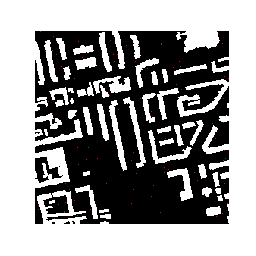
\includegraphics[width=\linewidth]{images/Berlin_1_256-71-5-label1.png}
    \end{minipage}
    \hfill
    \begin{minipage}[c]{0.4\linewidth}
        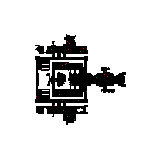
\includegraphics[width=\linewidth]{images/ht_chantry-31-1-label0.png}
    \end{minipage}%
\caption{Two sample MAPF problems represented as images. TODO: Adjust position at paper}
\label{fig:2}
\end{figure}

We use VGG-16 (\cite{simonyan2014very}), with the following different modifications: 1. Classification - adding classification head with the number of algorithms. \Roni{What is this?} Targets are one-hot-vector encoding of the relevant algorithm. 2. Regression - Adding regression output for each algorithm. Targets are log runtime for each algorithm on the relvant problem. 3. Multi Task - combination of classification and regression at the same network with loss weighting. 4. Multi input model - Concat our extracted features as input to the model.
\Roni{Items 3 and 4 are code names. I cannot figure out what you exactly did there. Important: need to focus on what we have results for.}

TODO: Should I ellaborate on all methods?

\subsection{GBDT models}
TODO: Details about sample weights, classification vs regression vs meta model?

\subsection{Feature Importance}
The ability to correctly interpret a model’s prediction is extremely important at the field of machine learning. Specifically, understanding why our model makes a certain prediction might reveal new knowledge about the solvers or support current assumptions on their weaknesses and strengths. At this section we will examine the feature importance of the manually extracted features we used to train our model. 
Due to the fact that our model is a complex model, we need to use a simpler explanation model, which is an interpretable approximation of our original complex model. Other techniques, such as adding interpretability constraints to the model, are usually costly in terms of accuracy, therefore at this paper we don't investigate them,

In order to compute the importance of each feature to the model, we used \textit{TreeExplainer} method, as defined by \cite{lundberg2019explainable}. \textit{TreeExplainer} is based on a local explanation method, thus combining local explanations from many samples in order to gain global model insights. 
The local explanations computed based on SHapley Additive exPlanation (SHAP) values (\cite{lundberg2017unified}). The basic intuition of how to compute \textit{Shapely} values is to find the average of the marginal contributions across all permutations for a given feature. 

Further information on techniques about interpretable machine learning has been recently made \cite{du2018techniques}.

Using TreeExplainer method, we compute the Shapley value for each feature at every sample on all labels. In order to gain a global understanding of the impact each feature made on the model, we do the following steps:
1. Compute the mean impact each feature had on the labels for every sample.
2. Compute the mean impact each feature had on all samples.

\begin{figure}[h]
    \centering
    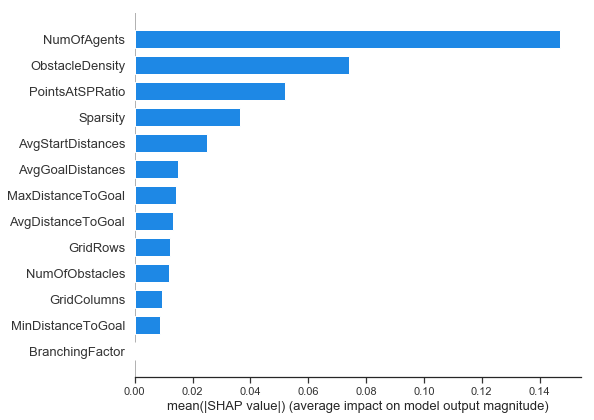
\includegraphics[width=0.5\textwidth]{Charts/mean_all_classes.png}
    \caption{Feature importance calculated using Shapley values. Features are sorted by their importance at y-axis. X-axis is the mean impact on model output, i.e. mean probability impact.}
    \label{fig:FeatureImportance}
\end{figure}

We can see that, as expected, the number of agents is highly influential. 
Furthermore, It can be seen that features that describe the map density (ObstacleDensity, PointsAtSPRatio, Sparsity, AvgStartDistances, AvgGoalDistances) have high impact also. 
Yet, some features, those describing the grid (rows and columns) and other quantitative measures (number of obstacles, branching factor) were not as helpful.

% As described above, our regression model consists of K regression models (where K is the number of algorithms, i.e. K=6). Here, we describe the feature importance for each regression model and use the results to enhance current assumptions about the different MAPF solvers we used.


\begin{center}
\begin{table}[t]
 \begin{tabular}{||c c c c||} 
 \hline
 Model & Accuracy & Coverage & Sum of costs \\ [0.25ex] 
 \hline
%  \hline
 Random & 16.33\% & 70.55\% & 13215 \\ 
 \hline
 EPE\astar & 11.81\% & 79.08\% & 9871 \\
 \hline
 MA-CBS & 26.34\% & 52.56\%	& 19952 \\
 \hline
 ICTS & 10.06\%	& 77.73\% & 10570 \\
 \hline
 \astar & 0.41\% & 73.08\% & 12459 \\
 \hline
 CBS & 0.43\% & 59.04\% & 17447 \\
 \hline
 CBS-H & 50.95\% & 83.12\% & 8016 \\ [0.25ex]
 \hline
%  \hline
 Oracle & 100.00\% & 100.00\% & 1649 \\
 \hline
 GBDT Regression & 51.09\%	& 82.21\% & 8410 \\
 \hline 
 GBDT Classification & 65.75\% & 93.13\% & 4307 \\
 \hline
 CNN Regression & 51.43\% & 88.21\% & 6210 \\ 
 \hline
 CNN Classification & 54.73\% & 91.01\% & 5122 \\
 \hline
 
\end{tabular}
\label{table:2}
\caption{Results of GDBT models}
\end{table}
\end{center}

\begin{figure}[h]
    \centering
    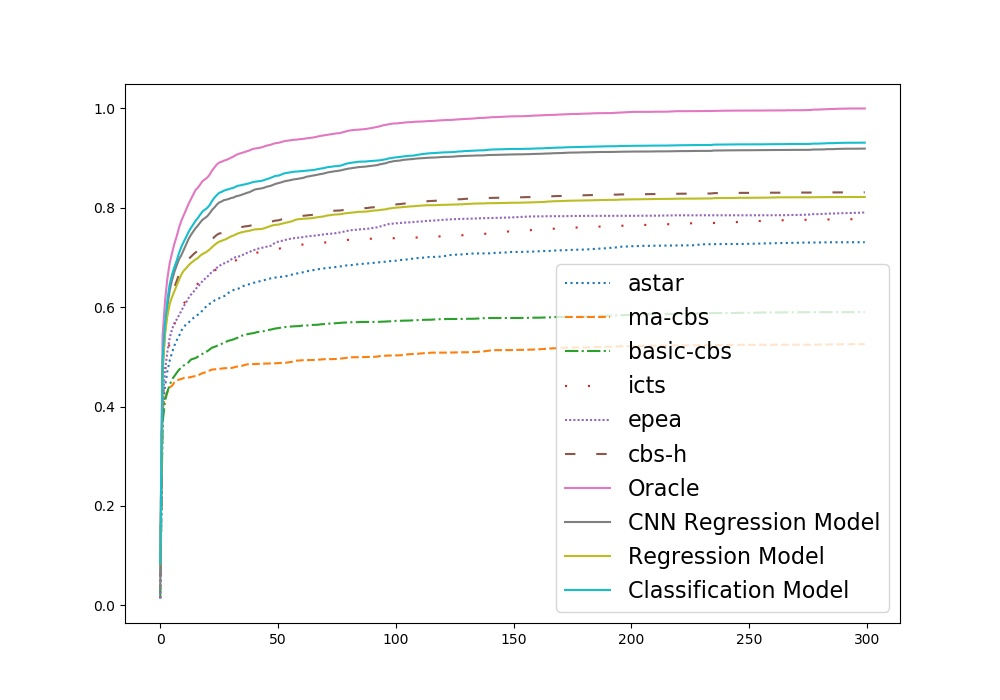
\includegraphics[width=0.5\textwidth]{images/all-cactus.jpg}
    \caption{Every solver (including the optimal solver and the algorithm selection ML model) is a line on the graph. X axis represent the time in seconds and y-axis represent the coverage metric. It is clear that the coverage using the ML Model is very close to the coverage of the oracle.}
    \label{fig:3}
\end{figure}

% \begin{figure}[h]
%     \centering
%     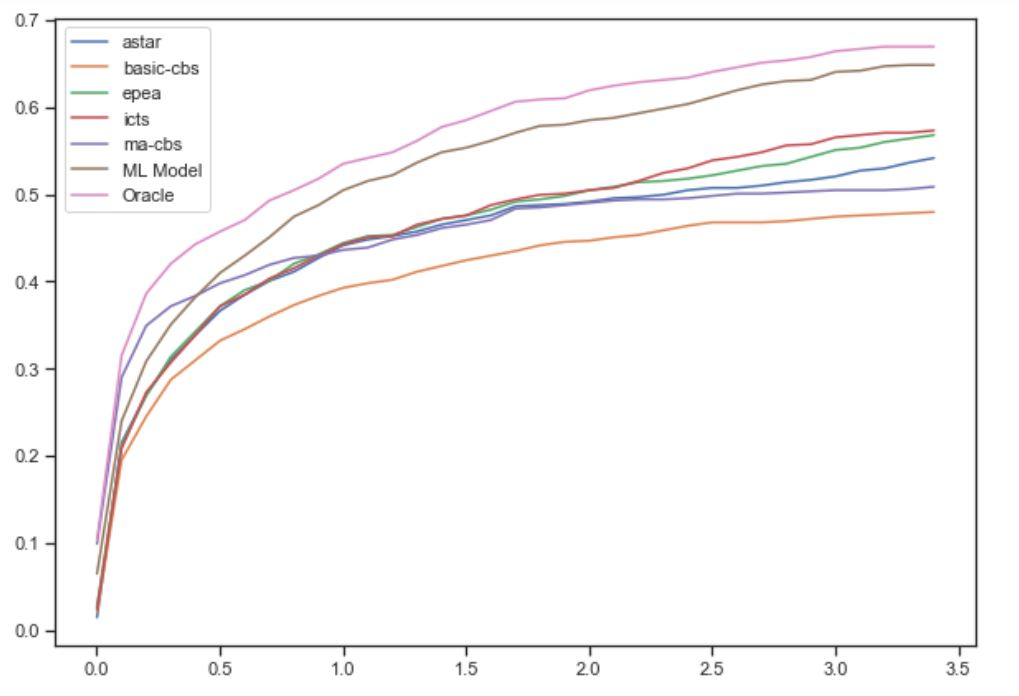
\includegraphics[width=0.5\textwidth]{images/coverage_cactus_limit_3500.jpg}
%     \caption{As in Figure 3 but this time zoomed in to 0-3.5 seconds range. This graph emphasize the behavior of Meta Agent CBS on Moving AI dataset and reveals the reason of the mismatch between it's accuracy and coverage metrics. We can see that although MA-CBS is a fast solver for easy problems, the other solvers are likely to solve those problems too. But for harder problems, while other solvers will slowly solve, MA-CBS will fail more often. }
%     \label{fig:4}
% \end{figure}

\begin{figure}[h]
    \centering
    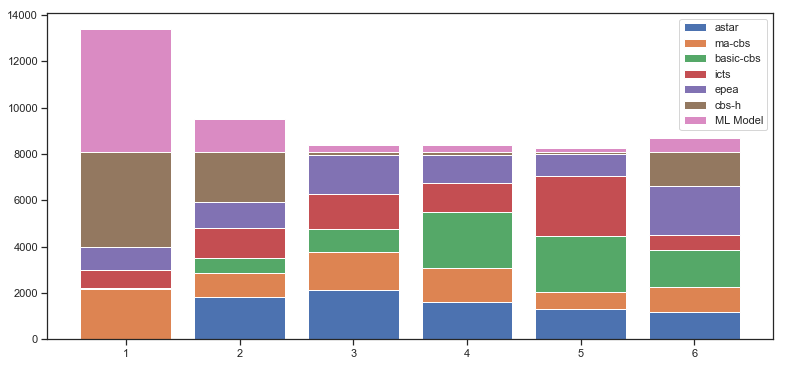
\includegraphics[width=0.5\textwidth]{images/stacked_bar_rankings_with_ml.JPG}
    \caption{Same figure as Figure 1, but this time with the ranks of the classification model mirrored above the ranks.}
    \label{fig:}
\end{figure}
\Roni{The above figure would have been better if you added the classification like all others. So it is also always sums to one. Otherwise, the difference with CBS-H is not clear.}

\subsection{Results per map type}
In order to gain deeper understanding about the solvers we did the same process for subsets of the data per map types. The types of map problems existed in the benchmark described at sub section 4.1. 

\begin{center}
\begin{table}[t]
 \begin{tabular}{||c c c c c c c||} 
 \hline
 Model & City & Game & Empty & Maze & Random & Room \\ [0.25ex] 
 \hline
%  \hline
 Random & 65.38\% & 68.51\% & 74.92\% & 84.04\% & 70.47\% & 82.97\% \\ 
 \hline
 EPE\astar & 66.87\% & 71.99\% & 94.95\% & 79.15\% & 88.04\% & 81.00\% \\ 
 \hline
 MA-CBS & 45.85\% & 49.23\% & 57.75\% & 77.52\% & 50.90\% & 68.34\% \\ 
 \hline
 ICTS & 70.89\% & 72.08\% & 83.60\% & 81.76\% & 85.86\% & 82.75\% \\ 
 \hline
 \astar & 65.69\% & 68.64\% & 85.00\% & 77.52\% & 74.21\% & 78.17\% \\ 
 \hline
 CBS & 55.33\% & 55.57\% & 59.60\% & 86.97\% & 55.02\% & 84.93\% \\ 
 \hline
 CBS-H & 91.34\% & 90.68\% & 67.45\% & 99.02\% & 71.28\% & 96.29\% \\ 
 \hline
%  \hline
 XGBoost Regression & 86.40\% & 89.68\% & 68.86\% & 96.74\% & 69.28\% & 91.05\% \\ 
 \hline
 XGBoost Classification & 87.07\% & 92.22\% & 90.24\% & 97.07\% & 90.09\% & 96.29\% \\ 
 \hline
 CNN Regression & 77.33\% & 91.99\% & 96.10\% & 94.14\% & 87.53\% & 87.55\% \\ 
 \hline
 CNN Classification & 91.34\% & 90.67\% & 88.13\% & 99.02\% & 90.84\% & 96.28\% \\ 
 \hline
\end{tabular}
\label{table:2}
\caption{Coverage Results of models per map type  }
\end{table}
\end{center}

\begin{center}
\begin{table}[t]
 \begin{tabular}{||c c c c c c c||} 
 \hline
 Model & City & Game & Empty & Maze & Random & Room \\ [0.25ex] 
 \hline
%  \hline
 Random & 16.07\% & 17.38\% & 17.74\% & 17.59\% & 17.32\% & 20.96\% \\ 
 \hline
 EPE\astar & 9.17\% & 5.43\% & 17.36\% & 0.00\% & 22.37\% & 5.68\% \\ 
 \hline
 MA-CBS & 21.69\% & 22.26\% & 43.52\% & 23.78\% & 23.61\% & 18.12\% \\ 
 \hline
 ICTS & 1.24\% & 8.05\% & 18.63\% & 5.21\% & 15.26\% & 12.88\% \\ 
 \hline
 \astar & 0.05\% & 0.05\% & 0.83\% & 0.00\% & 0.87\% & 0.87\% \\ 
 \hline
 CBS & 0.10\% & 0.72\% & 0.13\% & 0.98\% & 0.25\% & 1.75\% \\ 
 \hline
 CBS-H & 67.75\% & 63.48\% & 19.53\% & 70.03\% & 37.63\% & 60.70\% \\ 
 \hline
 XGBoost Regression & 12.26\% & 18.09\% & 10.08\% & 8.79\% & 9.90\% & 9.60\% \\ 
 \hline
 XGBoost Classification & 71.95\% & 87.23\% & 78.18\% & 67.41\% & 51.21\% & 66.59\% \\ 
 \hline
 CNN Regression & 56.44\% & 62.08\% & 43.39\% & 63.84\% & 37.81\% & 45.85\% \\ 
 \hline
 CNN Classification & 67.74\% & 63.48\% & 28.97\% & 70.03\% & 47.47\% & 60.69\% \\ 
 \hline
\end{tabular}
\label{table:2}
\caption{Accuracy Results of GDBT models on city-like MAPF maps }
\end{table}
\end{center}

\begin{figure}[h]
    \centering
    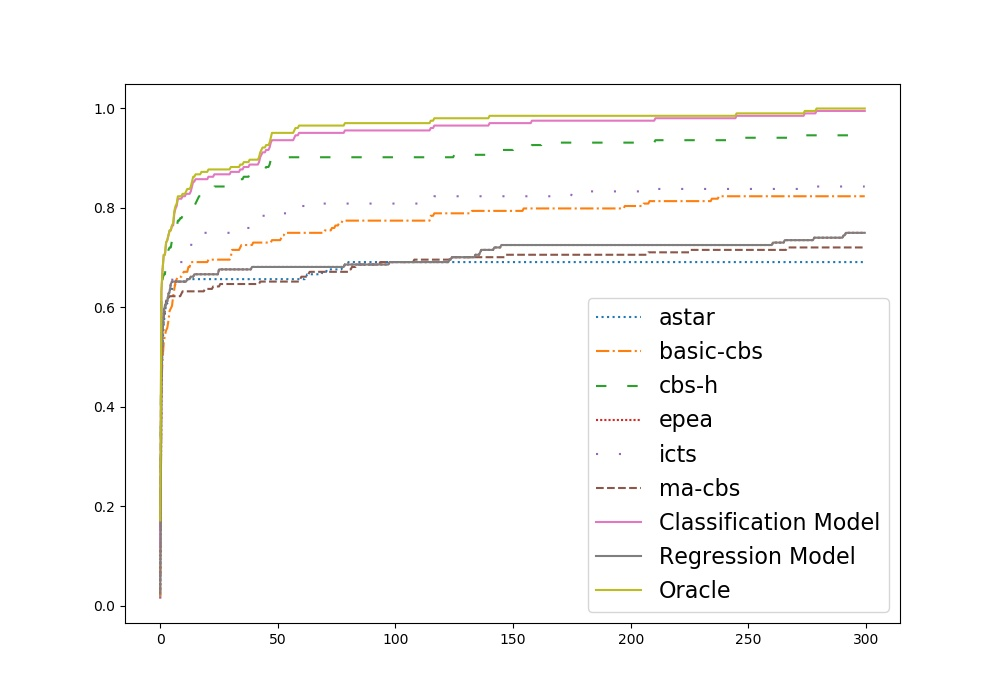
\includegraphics[width=0.5\textwidth]{images/maze-cactus.jpg}
    \caption{Maze maps - cactus graph with ML classification model}
    \label{fig:3}
\end{figure}

\begin{figure}[h]
    \centering
    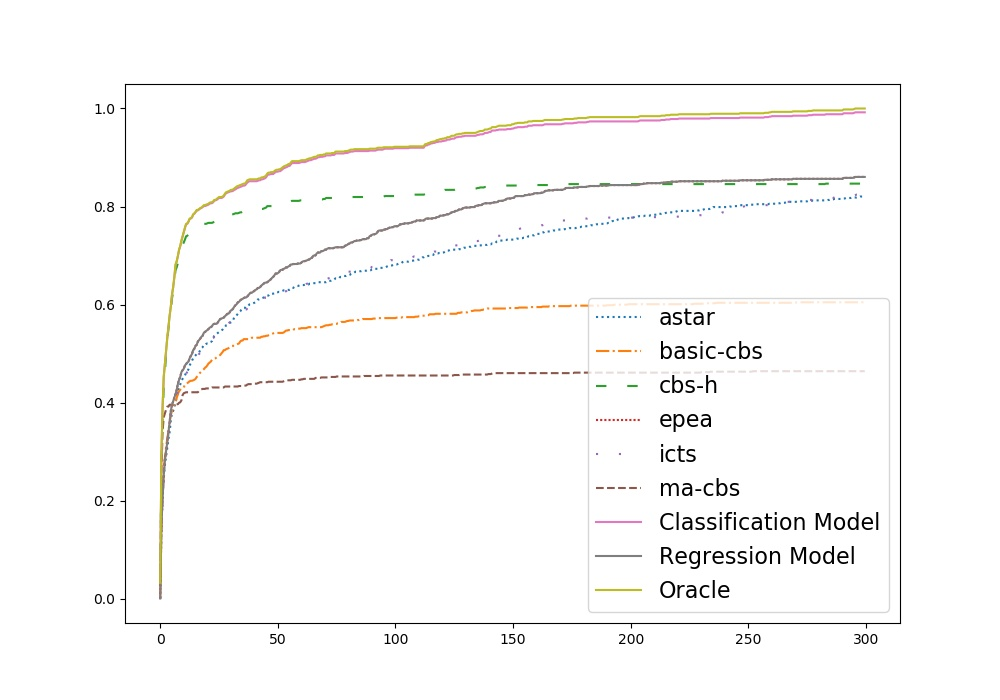
\includegraphics[width=0.5\textwidth]{images/city-cactus.jpg}
    \caption{City maps - cactus graph with ML models}
    \label{fig:3}
\end{figure}

\begin{figure}[h]
    \centering
    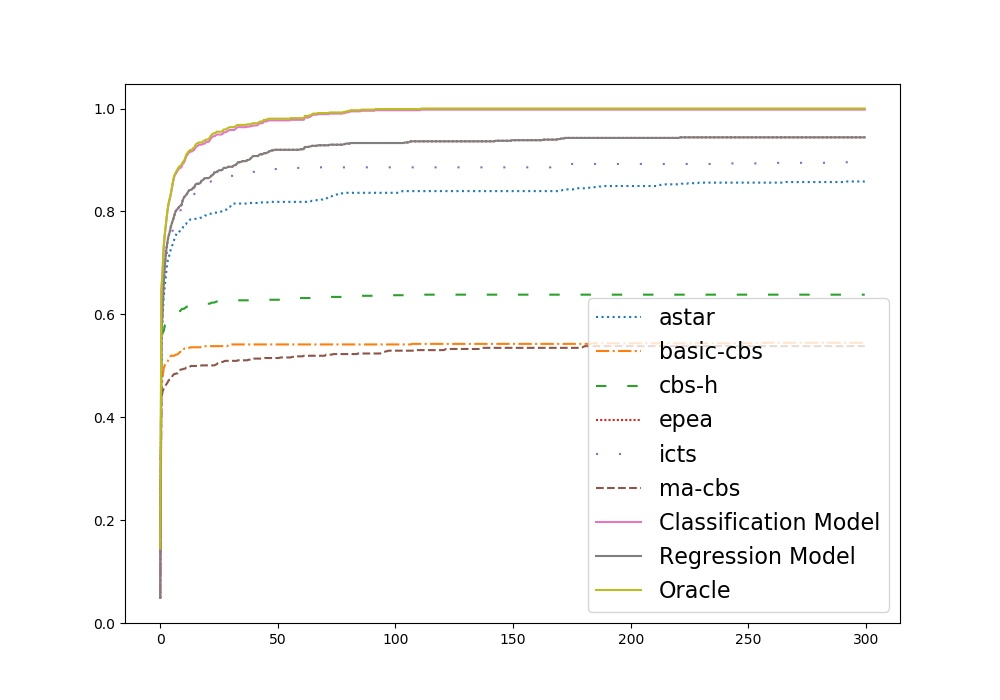
\includegraphics[width=0.5\textwidth]{images/empty-cactus.jpg}
    \caption{Empty maps - cactus graph with ML models}
    \label{fig:3}
\end{figure}

\begin{figure}[h]
    \centering
    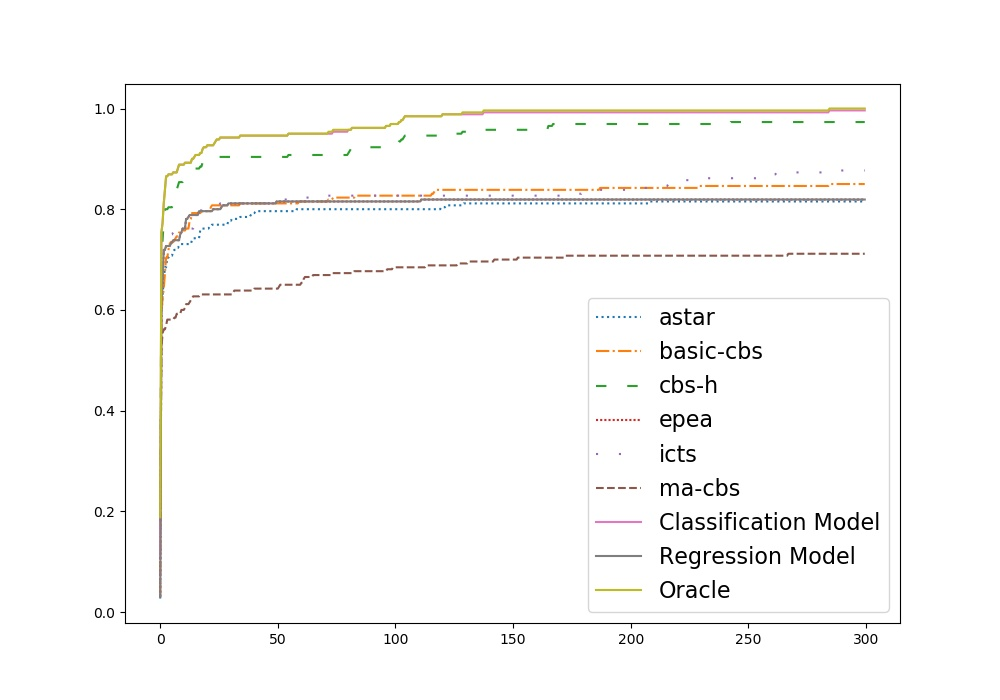
\includegraphics[width=0.5\textwidth]{images/room-cactus.jpg}
    \caption{Room maps - cactus graph with ML models}
    \label{fig:3}
\end{figure}

\begin{figure}[h]
    \centering
    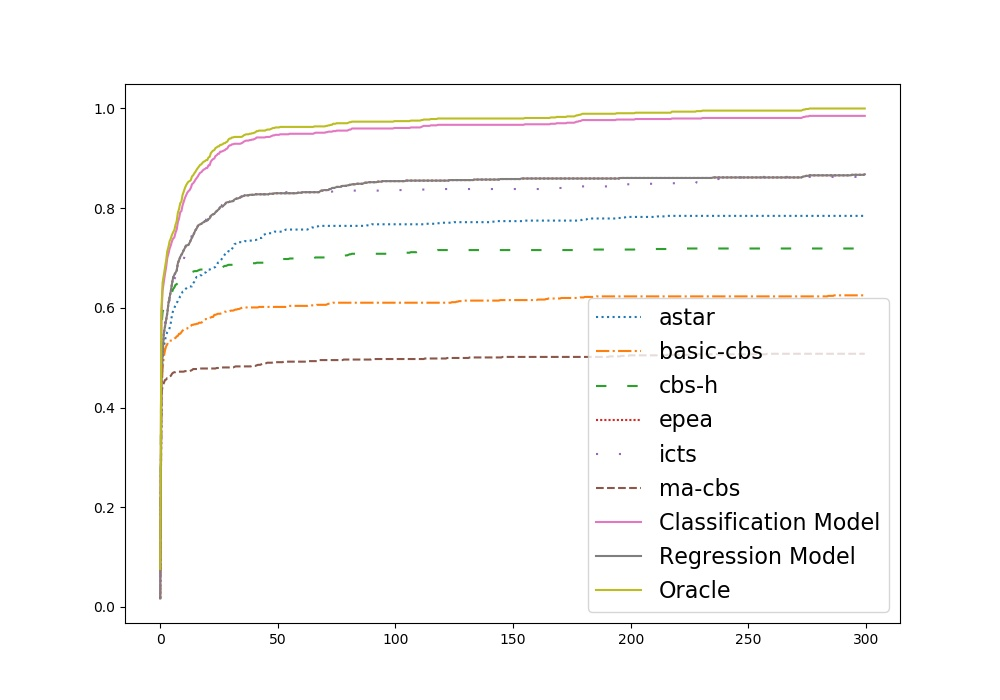
\includegraphics[width=0.5\textwidth]{images/random-cactus.jpg}
    \caption{Random maps - cactus graph with ML models}
    \label{fig:3}
\end{figure}

\begin{figure}[h]
    \centering
    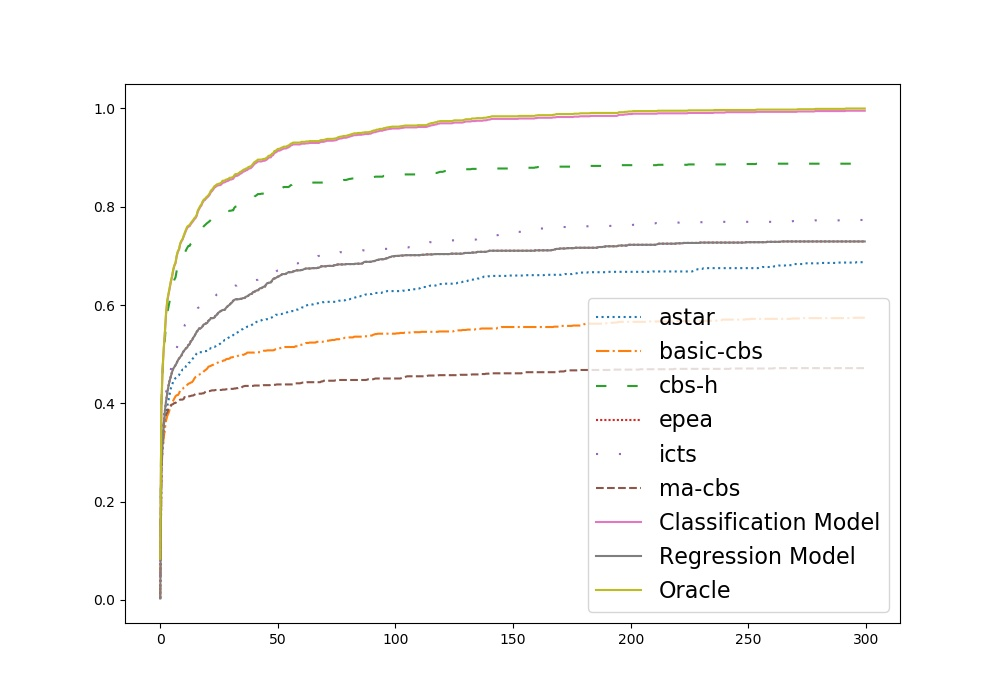
\includegraphics[width=0.5\textwidth]{images/game-cactus.jpg}
    \caption{Game maps - cactus graph with ML models}
    \label{fig:3}
\end{figure}



\section{Conclusion and Future Work}
At this paper we showed how machine learning techniques can be used to automatically select classic MAPF algorithm using only a small set of hand crafted features. Utilizing algorithm selection techniques to classical MAPF might lead us to develop specialized algorithms suited for a subset of MAPF problems, and combine them using machine learning models in order to create a dominant solver. 

TODO: Add discussion about using CNN for solving MAPF algorithm selection  - 1. Might work in cases such as \cite{sigurdson2019deep} where each map is dense with 300+ agents, but with small (~50) num of agents it is highly non-trivial for the network to distinguish each agent. Futhermore, no context of the path (relation between start and goal) has been taken into consideration, which we believe might be crucial.
2. Can not utilize transfer learning
3. Can't scale naively to non regular grid MAPF problems 

Yet, our model still uses hand-crafted features. We believe that there is a place for future work that will utilize deep learning to learn a feature representation from the graph, thus enable the expansion of algorithm selection to other multi agent path finding fields, which all can be described as a graph. Also, we believe that gaining insight about how the model achieve the results we have obtained, might lead to new discoveries about the weakness of current solvers.


\section{Appendix}
\resizebox{\columnwidth}{!}{
    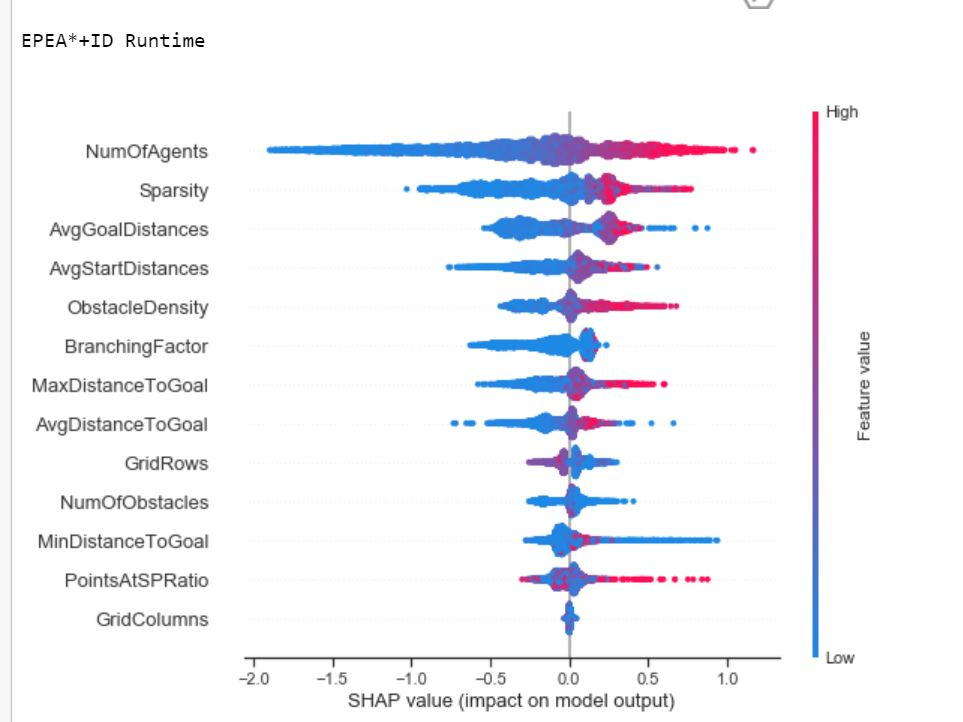
\includegraphics[width=0.5\textwidth]{EPEA.JPG}
        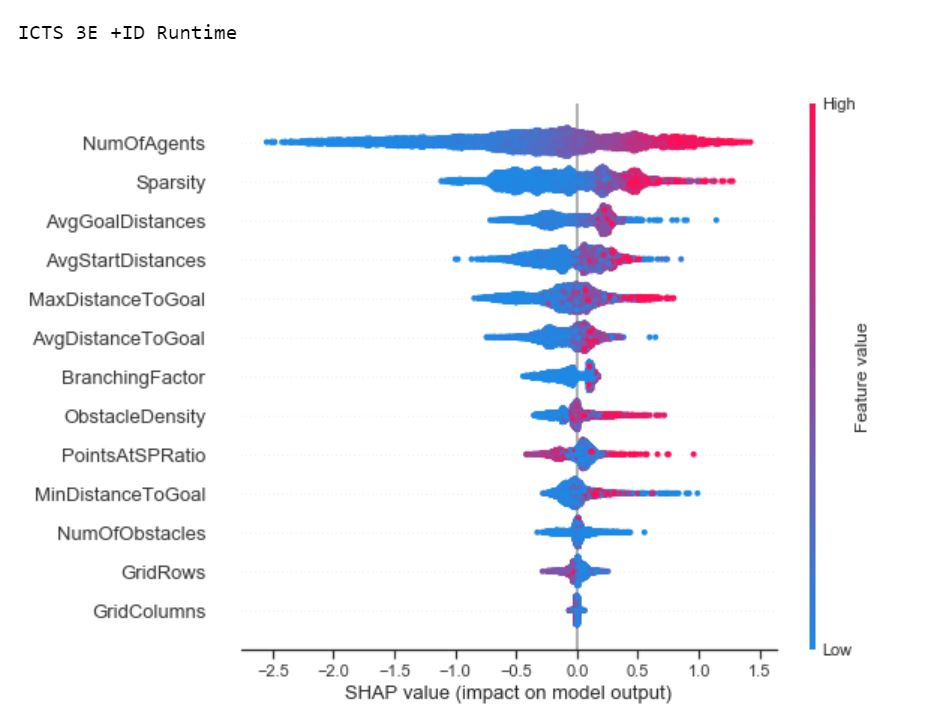
\includegraphics[width=0.5\textwidth]{ICTS.JPG}
    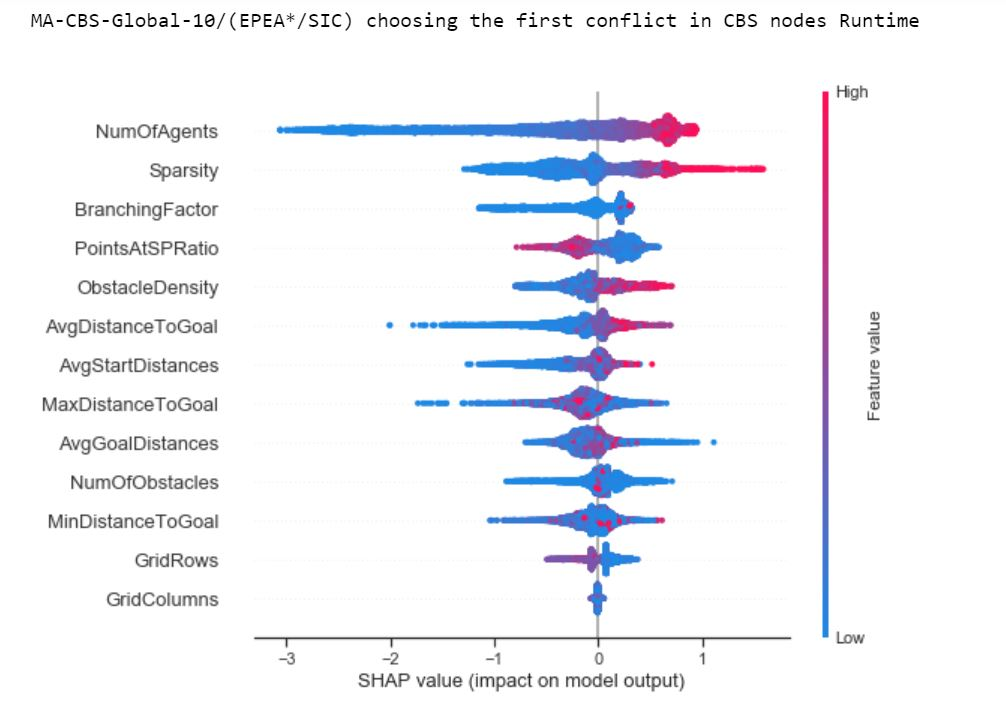
\includegraphics[width=0.5\textwidth]{MA-CBS.JPG}
}
\begin{figure}[h]
    \centering
    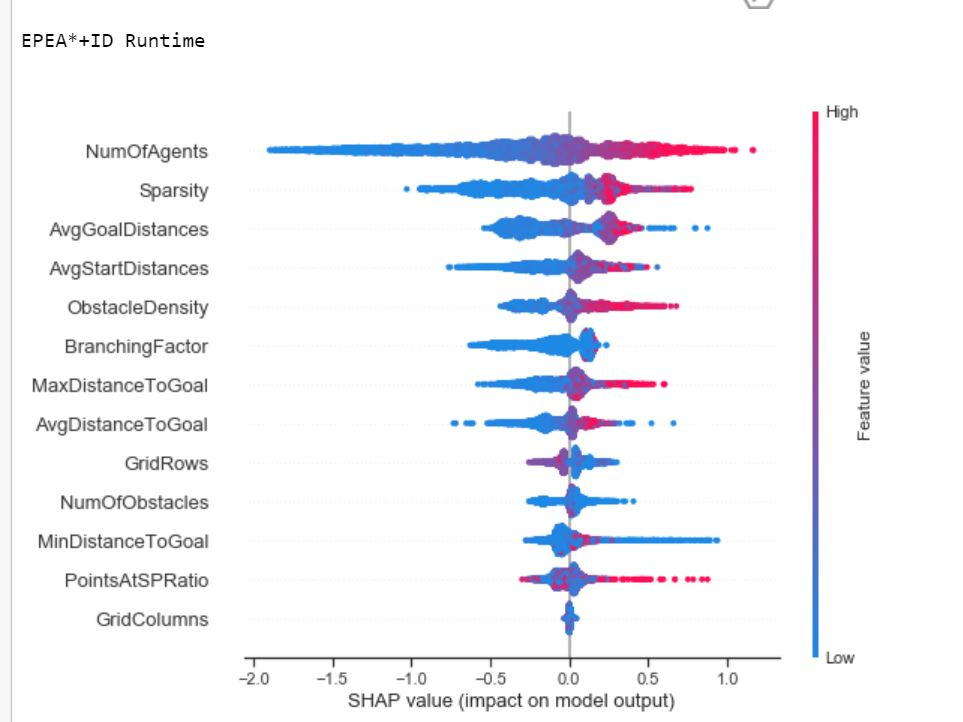
\includegraphics[width=0.5\textwidth]{EPEA.JPG}
    \caption{EPEA shap feature importance}
    \label{fig:3}
\end{figure}

\begin{figure}[h]
    \centering
    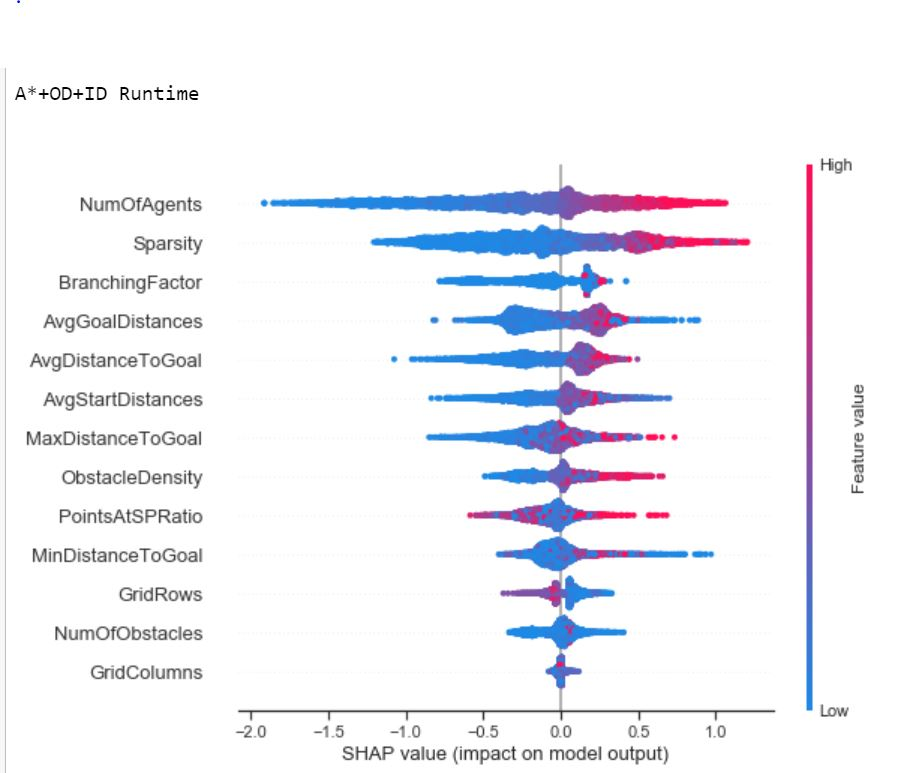
\includegraphics[width=0.5\textwidth]{ASTAR.JPG}
    \caption{A* shap feature importance}
    \label{fig:3}
\end{figure}
\begin{figure}[h]
    \centering
    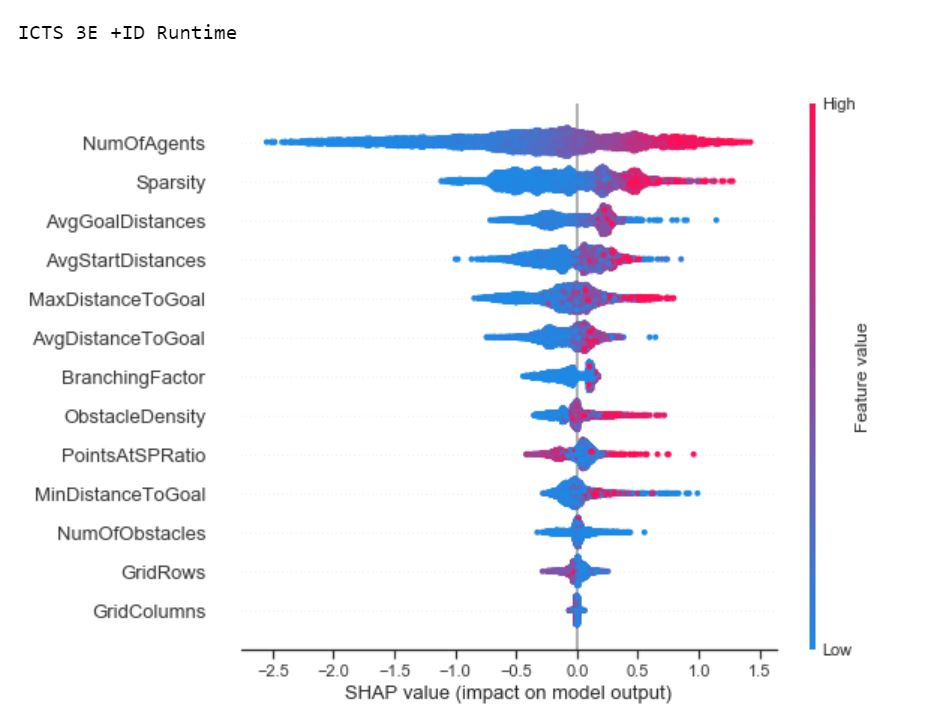
\includegraphics[width=0.5\textwidth]{ICTS.JPG}
    \caption{ICTS shap feature importance}
    \label{fig:3}
\end{figure}
\begin{figure}[h]
    \centering
    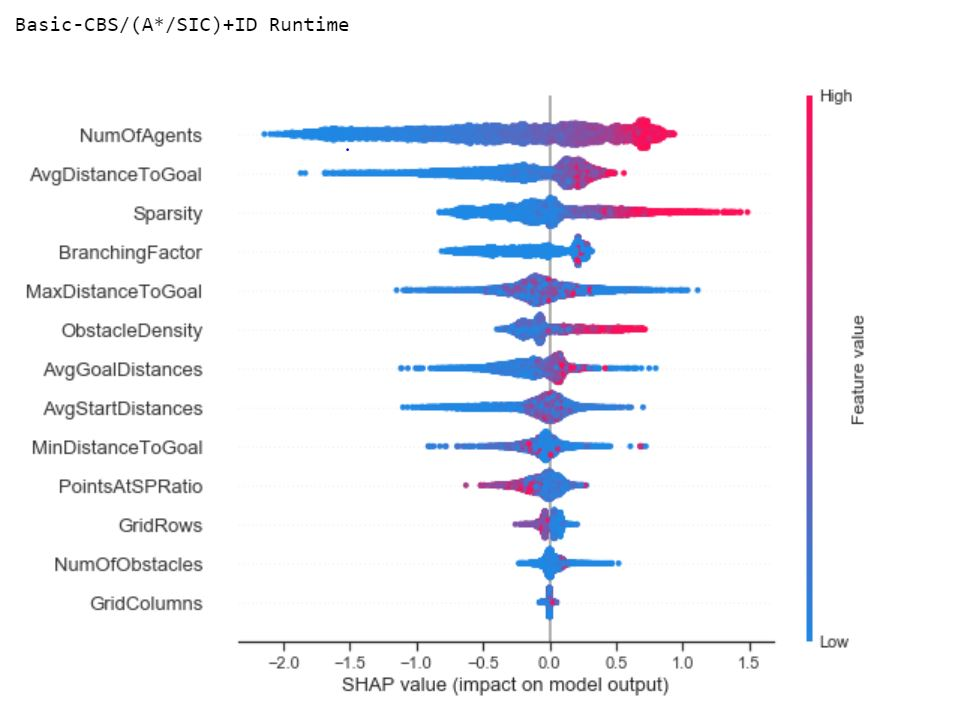
\includegraphics[width=0.5\textwidth]{CBS.JPG}
    \caption{CBS shap feature importance}
    \label{fig:3}
\end{figure}
\begin{figure}[h]
    \centering
    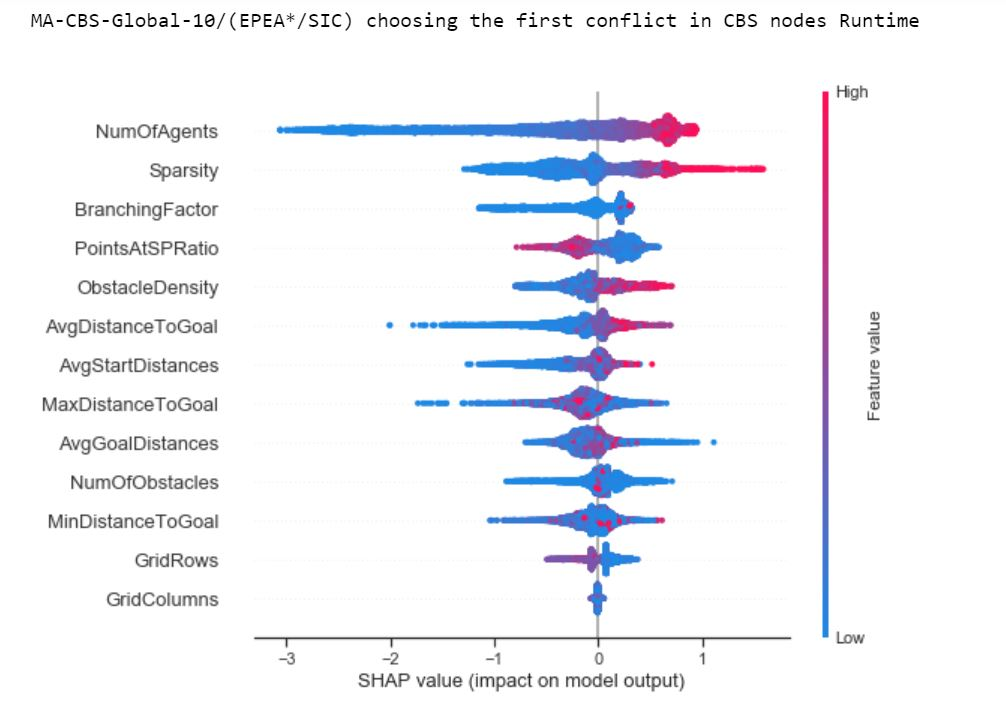
\includegraphics[width=0.5\textwidth]{MA-CBS.JPG}
    \caption{MA-CBS shap feature importance}
    \label{fig:3}
\end{figure}

\begin{figure}[h]
    \centering
    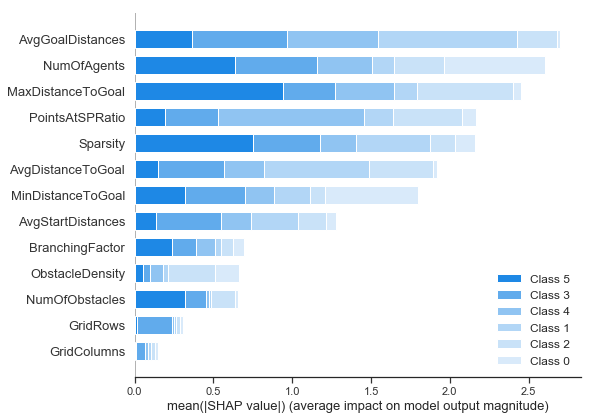
\includegraphics[width=0.5\textwidth]{clf-shap.png}
    \caption{classification shap feature importance}
    \label{fig:3}
\end{figure}

%\balance
% \bibliographystyle{aaai}
% \bibliography{ref}
\medskip
\printbibliography


%% The file named.bst is a bibliography style file for BibTeX 0.99c
%\bibliographystyle{aaai}
%\bibliography{sam}

\end{document}